

%!TEX root = ../Notes.tex
\section{Continuity in Topological Spaces} 
\begin{definition}
	Let $(X_1,F_1)$ and $(X_2,F_2)$ be topological spaces and $f: X_1 \to X_2$. We say $f$ is \textbf{continuous} if and only if for every $U \in F_2$, $f^{-1}(U)\in F_1$. 
\end{definition}
\begin{smallfact}
	Let $(X_1,F_1)$ and $(X_2,F_2)$ and $(X_3,F_3)$ be topological spaces, $f: X_1 \to X_2$ and $f: X_2 \to X_3$ be continuous functions. Then $g \circ f: X_1 \to X_3$ is continuous. 
\end{smallfact}
\begin{proof}
	Let $U \in F_3$. Then $g^{-1}(U) \in F_2$ because $g$ is continuous, and $f^{-1}(g^{-1}(U)) \in F_1$ because $f$ is continuous. Therefore $(g \circ f)^{-1}(U) \in F_1$. Thus $g\circ f$ is continuous. 
\end{proof}
\begin{theorem}
	Let $X$, $Y$ be topological spaces and $f: X \to Y$. Then $f$ is continuous if and only if for every closed set C in Y, $f^{-1}(C)$ is closed in X. 
\end{theorem}
\begin{proof}
	\begin{itemize}
		\item [$(\Rightarrow)$] Suppose $C$ is closed in $Y$. Then $Y\setminus C$ is open, implying that $f^{-1}(Y\setminus C)$ is open in $X$. Since $f^{-1}(Y\setminus C)= \{ x \in X\ |\ f(x) \in Y\setminus C\} = \{ x \in X\ |\ f(x) \notin C \}$ and $X\setminus f^{-1}(C)= \{ x \in X\ |\ f(x) \notin C \}$, we have the desired results. 
		\item [$(\Leftarrow)$] This is exactly like the analogous proof for open sets. 
	\end{itemize}
\end{proof}

This is nice, because sometimes it's easier to work with closed sets than with open sets. 
\begin{definition}
	Let $X$ and $Y$ be topological spaces, and let $f:X\to Y$. 
	\begin{enumerate}
		\item If for every open set $U\subseteq X$, $f(U)$ is open in $Y$, then $f$ is \textbf{open}. 
		\item If for every closed set $U\subseteq X$, $f(U)$ is closed in $Y$, then $f$ is \textbf{closed}. 
	\end{enumerate}
\end{definition}

This is sort of like continuity, except that we care about the image of sets instead of their preimages.

Example time! 
\begin{example}
	Let $F$ be the half-open topology on $\R$, and define a function
	\[{f:(\R,F)\to(\R,\text{usual})}\qquad\text{ by }f(x) = x\]
\end{example}
\begin{itemize}
	\item Is $f$ continuous? Yes! An open set in $(\R, \text{usual})$ is a union of intervals of the form $(a,b)$. We know that $f^{-1}\big((a,b)\big) = (a,b)$, which is open in $F$. 
	\item Is $f$ open? No. Take any $U = [a,b) \in F$. Then $f(U) = [a,b)$, which is not open in $(\R, \text{usual})$. 
	\item Is $f$ closed? Also no, since $f\big([a,b)\big) = [a,b)$ is not closed in $(\R, \text{usual})$. 
\end{itemize}

\section{Homeomorphisms} Let's define a notion of equivalency for topological spaces. 
\begin{definition}
	Let $(X_1,F_1)$ and $(X_2,F_2)$ be topological spaces, and let $f:X_1\to X_2$ be continuous, bijective, and open. Then $f$ is a \textbf{homeomorphism}, and $X_1$ and $X_2$ are \textbf{homeomorphic} (denoted by $X_1 \cong X_2$). 
\end{definition}
\begin{example}
	Let $I = [0,1]$ and $X = I\times I\subset\R^2$, under the usual metric for $\R^2$. Let \nobreak{$Y = \{ (x,y)\in\R^2 | x^2+y^2\le 1\} = D^2$} be the unit disk in $\R^2$. Question: Are $X$ and $Y$ homeomorphic? 
	
	Answer: Yes! Let's see how. 
\end{example}

Define the centers of $X$ and $Y$ to be $x$ and $y$, respectively. Fix some point $a$ on the boundary of $X$, and some $b$ on the boundary of $Y$ (that is, $a\in 
\partial X$ and $b\in
\partial Y$).

Define a function $f$ as follows: 
\begin{itemize}
	\item $f(x) = y$ 
	\item $f(a) = b$ 
	\item For $t\in 
	\partial X$, look at the distance along the boundary from $a$ to $t$. Then $f(t)$ is a point proportionally far along the boundary of $Y$. 
	\item For $s\in \text{int}(X)$, draw the ray connecting $x$ and $s$. Let $t$ be the point at which this ray intersects $ 
	\partial X$. Now, in $Y$, draw the ray connecting $y$ and $f(s)$. Then $s$ is mapped to a point on this ray that is proportionally far from $y$. 
\end{itemize}
The last two, in pictures:
\[ 
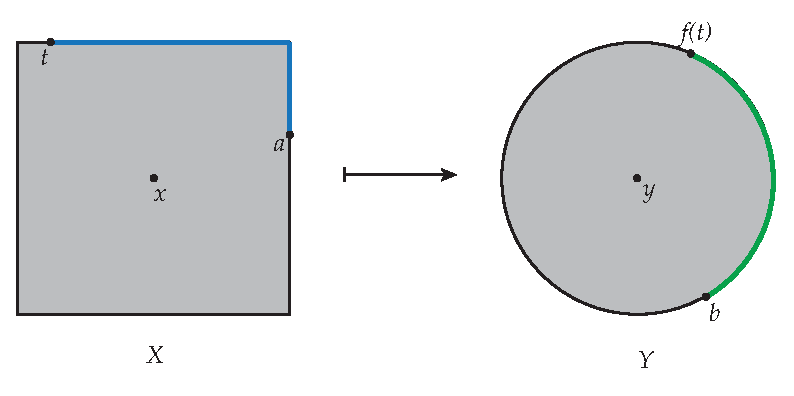
\includegraphics[width=360pt]{images/continuity_and_topology/square_circle_map_1}\]
\[ 
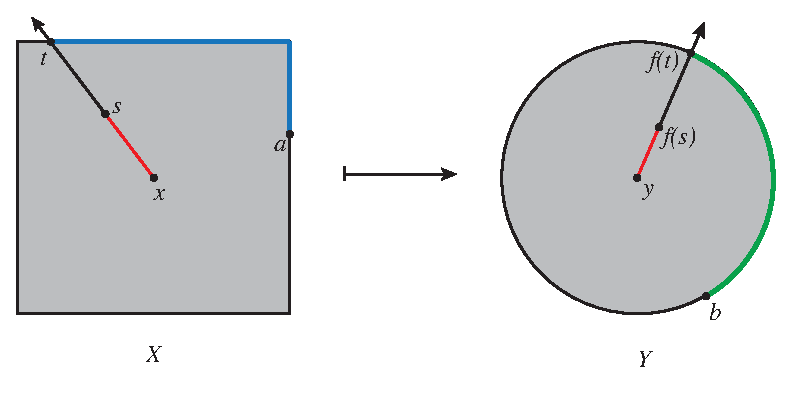
\includegraphics[width=360pt]{images/continuity_and_topology/square_circle_map_2}\]
\begin{itemize}
	\item Is this well-defined? 
	\begin{itemize}
		\item Yes! There is always exactly one point in $Y$ that can be mapped to be a point in $X$\footnote{This works because both a square and a circle are \emph{convex} shapes - for example, for all points $p,q\in X$, the line $\overline{pq}$ that connects $p$ and $q$ lies entirely within $X$. This also implies that $x$ and $y$ didn't actually have to be the exact \emph{centers} of $X$ and $Y$ respectively.}. 
	\end{itemize}
	\item Is this a bijection? 
	\begin{itemize}
		\item Yes! The inverse is defined identically, so it would make sense for this to be a bijection. Also, consider the images of concentric squares centered on $x$ under $f$: they are mapped to disjoint concentric circles centered on $y$. 
	\end{itemize}
	\item Is $f$ continuous and open? 
	\begin{itemize}
		\item Yes! Intuitively, it's easy to see that an open set in $X$ is mapped to an open set in $Y$, and that the preimage of an open set in $Y$ is open. 
	\end{itemize}
\end{itemize}

Question: Can we extend this to (some) non-convex regions? 

Answer: Sure. Just divide up the non-convex region into smaller regions. Actually, a subregion will work as long as there is some point in its interior such that any ray from that point intersects the subregion's boundary exactly once.

However, there are limits to this: for example, a donut is \emph{not} homeomorphic to a circle. This is hard to show; we'll see a proof later.

There are also some homeomorphisms that we might find unsettling. For example, a knot in $\R^3$ and the unit circle $S^1 = \{ (x,y)\in\R^2 | x^2+y^2 = 1\}$ are homeomorphic; the argument works exactly like the one used for $ 
\partial X$ when showing that a square and circle are homeomorphic (above). It turns out that, while the knot and circle are homeomorphic, their complements are not. 
\begin{example}
	Define a function $f:[0,1)\to S^1$ by
	\[ f(t) = \big( \cos(2\pi t), \sin(2\pi t)\big) \]
\end{example}
This takes the interval and wraps it counterclockwise around the circle. 
\begin{itemize}
	\item Is this a bijection? 
	\begin{itemize}
		\item Yes! The interval wraps once around the circle; one end is open, so there is no overlap. 
	\end{itemize}
	
	\item Is $f$ continuous? 
	\begin{itemize}
		\item Yes! First we define an open ball in $S^1$ as $B_{\epsilon, S^1}(a) = \{x\in S^1\ |\ d(x,a) < \epsilon\}$. Then the preimage of every open ball in $S^1$ is an open interval, so $f$ is continuous. 
	\end{itemize}
	
	\item Is $f$ open? 
	\begin{itemize}
		\item No. Let $U = [0, 1/2)$, which is open in $[0,1)$. Sadly, its image is not open in $S^1$. 
	\end{itemize}
\end{itemize}
So this $f$ is not a homeomorphism.

\mbox{ }

We will show that $\R^2 \not\cong \R^3$ near the end of Chapter 3. This is difficult. 
\begin{example}
	Some non-examples of homeomorphisms: 
\end{example}
\begin{itemize}
	\item $\Q$ under the usual topology is not homeomorphic to $\R$ under the usual topology, since there is no bijection between $\Q$ and $\R$. 
	\item $\R$ with the finite-complement topology ($FCT$) is not homeomorphic to $\R$ with the usual topology: 
	\begin{itemize}
		\item Suppose that there is some homeomorphism $f:(\R, FCT)\to(\R,\text{usual})$. Let $U = (0,1)$. 
		\item Look at $f^{-1}(U)$ - it must be open, since $f$ is a homeomorphism. 
		\item It is definitely not equal to $\emptyset$, since $U\ne\emptyset$. 
		\item It is also not $\R$, since $f$ is a bijection. 
		\item So $\R\setminus f^{-1}(U)$ must be finite. But $\R\setminus U$ is not finite. 
		\item Because $f$ is a bijection, this is a contradiction. 
		\item Therefore, $(\R, FCT) \not\cong (\R, \text{usual})$. 
	\end{itemize}
\end{itemize}
